
\documentclass[10pt,landscape]{scrartcl}

\usepackage[english]{babel}
% \usepackage[ngerman]{babel}
\usepackage[utf8]{inputenc}

\usepackage{lmodern}

\usepackage{ifthen}

\usepackage{graphicx}
% \usepackage{pstricks}
% \usepackage{relsize}
% \usepackage[decimalsymbol=comma,exponent-product = \cdot, per=frac]{siunitx}
% \sisetup{range-phrase=\,bis\,}

\usepackage{xargs}
\usepackage{calc}
\usepackage{amsmath}
\usepackage{amsfonts}
\usepackage{mathtools}
\usepackage{amssymb}

\usepackage{cancel}
\usepackage{trfsigns}
\usepackage{array}
\usepackage{enumerate}
\usepackage{enumitem}

\usepackage{caption}
\usepackage{subcaption}

\usepackage{multicol}

\usepackage{pdflscape}
\usepackage[table]{xcolor}

\usepackage{float}

%%%%%%%%%%%%%%%%%%%%%%%%%%%%%%%%%%%%%%%%%%%%%%%%%%%%%%%%%%%%%%%%%%%%%%%%%%%%%%%%
\newboolean{WITHPSTRICKS}
\setboolean{WITHPSTRICKS}{false}


\newcommand{\PROFESSOR}{Prof.\ Dr.\ Thomas Carraro}
\newcommand{\ASSISTANT}{\setlength{\tabcolsep}{0pt}\begin{tabular}{l}Dr.\ Frank Gimbel\\Janna Puderbach\end{tabular}}

\newcommand{\Jahr}{2022}
% \newcommand{\Trimester}{HT}
\newcommand{\Trimester}{WT}
\newcommand{\Kurs}{Mathematik II}
\newcommand{\TYPE}{Aufgabenblatt}
\newcommand{\BLATT}{0}
\newcommand{\TOPIC}{Wiederholung}

%%%%%%%%%%%%%%%%%%%%%%%%%%%%%%%%%%%%%%%%%%%%%%%%%%%%%%%%%%%%%%%%%%%%%%%%%%%%%%%%
\newboolean{mitLoes}
\setboolean{mitLoes}{false}
%  \setboolean{mitLoes}{true}

%%%%%%%%%%%%%%%%%%%%%%%%%%%%%%%%%%%%%%%%%%%%%%%%%%%%%%%%%%%%%%%%%%%%%%%%%%%%%%%%


%\setboolean{WITHPSTRICKS}{false}
\setboolean{WITHPSTRICKS}{true}


\usepackage{tikz}
\usetikzlibrary{arrows,automata,backgrounds,calendar,decorations.pathmorphing,fadings,shadings,calc,intersections}
\usetikzlibrary{decorations.pathreplacing}
\usetikzlibrary{decorations.shapes}
\usetikzlibrary{decorations.footprints}
\usetikzlibrary{decorations.text}
\usetikzlibrary{positioning}
\usetikzlibrary{through}
\usepackage[utf8]{inputenc}


\ifthenelse{\boolean{WITHPSTRICKS}}{%
\usepackage{auto-pst-pdf}
\usepackage{pstricks,pst-plot,pst-text}
}{}

\usepackage{pgfplots}

%%%%%%%%%%%%%%%%%%%%%%%%%%%%%%%%%%%%%%%%%%%%%%%%%%%%%%%%%%%%%%%%%%%%%%%%%%%%%%%%
\usepackage{mbdefAufgaben}

%%%%%%%%%%%%%%%%%%%%%%%%%%%%%%%%%%%%%%%%%%%%%%%%%%%%%%%%%%%%%%%%%%%%%%%%%%%%%%%%
\newboolean{mitErg}
%\setboolean{mitErg}{false}

%%%%%%%%%%%%%%%%%%%%%%%%%%%%%%%%%%%%%%%%%%%%%%%%%%%%%%%%%%%%%%%%%%%%%%%%%%%%%%%%
\newcounter{Aufg}
\setcounter{Aufg}{0}
\newcounter{Blatt}
\setcounter{Blatt}{1}

%%%%%%%%%%%%%%%%%%%%%%%%%%%%%%%%%%%%%%%%%%%%%%%%%%%%%%%%%%%%%%%%%%%%%%%%%%%%%%%%
%\usepackage{KopfEnglish}

% Seitenraender
%\textwidth = 285mm
%\textheight = 180mm
%\leftmargin 5mm
%\oddsidemargin = -20mm
%\evensidemargin = -20mm
%\topmargin = -25mm
%\parindent 0cm
%\columnsep 2cm

% % % Aufgabenstellung
% % % Schwierungkeitsgrad mit "e" , "f" oder "v" angeben
% % % "e" Einführung   
% % % "f" Festigung
% % % "v" Vertiefung  

\newcommand{\Aufgabe}[3][]{
\stepcounter{Aufg}
\subsubsection*{Aufgabe 
\arabic{Aufg}\ifthenelse{\equal{#1}{e}}{}{\ifthenelse{\equal{#1}{f}}{
$\!\!{}^\star$}{\ifthenelse{\equal{#1}{v}}{$^{\star\star}$}{}}}{: #2}}
{#3}
}
% % % Ergebnisse jeweils am Ende des Aufgabenblattes Anzeigen
\newcommand{\Ergebnisse}{}
\makeatletter
\newcommand{\Ergebnis}[1]{
	\g@addto@macro{\Ergebnisse}{#1}
}
\makeatother
\makeatletter
\newcommand{\ErgebnisC}[2]{
\@ifundefined{c@#1}
{\newcounter{#1}}
{}
\setcounter{#1}{\theAufg}

\ifthenelse{\boolean{mitErg}}{	\g@addto@macro{\Ergebnisse}{\subsubsection*{Ergebnisse zu Aufgabe \arabic{#1}:}
}%
	\g@addto@macro{\Ergebnisse}{#2}}{}
}
\makeatother


% % % Lösungen
\newcommand{\Loesung}[1]{
	\ifthenelse{\boolean{mitLoes}}
	{\subsubsection*{Lösung \arabic{Aufg}:}
		#1}
	{}
}
% % % % % % % % % % % % % % % % % % % % % % % % % % % % % % % % % % % % % % % % % % % % % % % % % % % % % %
% % % % % % % % % % % % % % % % % % % % % % % % % % % % % % % % % % % % % % % % % % % % % % % % % % % % % %
% % % % % % % % % % % % % % % % % % % % % % % % % % % % % % % % % % % % % % % % % % % % % % % % % % % % % %
\begin{document}
%\begin{twocolumn}
% % % % % % % % % % % % % % % % % % % % % % % % % % %

%%%%%%%%%%%%%%%%%%%%%%%%%%%%%%%%%%%%%%%%%%%%%%%%%%%%%%%%%%%%%%%%%%%%%%%%%%%%%%%%
% Set the TITLE of the sheet here:
%\uebheader{\Kurs}{\arabic{Blatt}}{\Trimester\,\Jahr}{\TOPIC}
%\uebheader{\Kurs}{\arabic{Blatt}}{\Trimester\,\Jahr}{\TOPIC}
%\uebheader{\Kurs}{\arabic{Blatt}}{\Trimester\,\Jahr}{\TOPIC}
%\ruleBig

\setboolean{mitErg}{false}
 \setboolean{mitErg}{true}


%%%%%%%%%%%%%%%%%%%%%%%%%%%%%%%%%%%%%%%%%%%%%%%%%%%%%%%%%%%%%%%%%%%%%%%%%%%%%%%%
% Set the INTRODUCTION section of the sheet here:
% \input{introduction.tex}

\textbf{Einführende Bemerkungen}

\begin{itemize}
\item Dieses Übungsblatt enthält Aufgaben angelehnt an die Klausuraufgaben.
\item Achten Sie darauf, dass Sie die Notation beherschen und die Aufgaben sauber Niederschreiben.
\item Vermeiden Sie die Verwendung von Taschenrechnern oder Online-Ressourcen.
\item Die mit einem Stern *) markierten (Teil-)Aufgaben werden im ISA-Kurs behandelt,  
k\"onnen und sollen aber auch von den Studierenden bearbeitet werden, die nicht am ISA-Kurs teilnehmen. 
Bitte laden Sie Ihre Lösungen im ILIAS hoch.
\end{itemize}

\ruleBig

%Mathe II Blatt 0
\Aufgabe[e]{Matrizen}{
Gegeben seien folgende Matrizen und Vektoren
\begin{center}
\begin{align*}
% 3x3 unit\"ar
&\vec A = 
    \frac{1}{\sqrt 2} \begin{pmatrix} 
    \operatorname{i} & 0 & -\operatorname{i} \\
    \operatorname{i} & 0 & \operatorname{i}\\
    0 & \sqrt{2} & 0\end{pmatrix}
     , \,
% 4x2
&\vec B = \begin{pmatrix}
    \operatorname{i} & 1\\
    -1 & -\operatorname{i}\\
    0 & 1\\
    2\operatorname{i} & 1
    \end{pmatrix}\, , \,
% 2x2 orthogonal
&\vec C = \begin{pmatrix}
    \frac{\sqrt{2}}{2} & \frac{\sqrt{2}}{2}\\
    -\frac{\sqrt{2}}{2} & \frac{\sqrt{2}}{2}
    \end{pmatrix}\, , \\
% 4x4 symmetrisch
&\vec D = \begin{pmatrix}
    1 & 2 & 3 & 4\\
    2 & 1 & 5 & 6\\
    3 & 5 & 1 & 7\\
    4 & 6 & 7 & 1
    \end{pmatrix}\, , \,
% 3x2
&\vec E = \begin{pmatrix}
    1 & 1\\
    1 & 0\\
    0 & 1
    \end{pmatrix} \, , \,
%
&\vec F = \begin{pmatrix}
    0 & \operatorname{i}\\
    -\operatorname{i} & 0
    \end{pmatrix}\\
% v_1 , v_2 
&\vec v_1 = \begin{pmatrix}
    \operatorname{i} \\ 1 - 2\operatorname{i} \\ 3
    \end{pmatrix}\, , \,
&\vec v_2 = \begin{pmatrix}
    1 -\operatorname{i} \\ -2 \\ -2 + \operatorname{i}
    \end{pmatrix}
\end{align*}
\end{center}
\begin{abc}
\item Welche Matrixprodukte und Matrix-Vektorprodukte sind definiert? (Zur Übung können Sie alle 
      Produkte berechnen.)
\item Erkl\"aren Sie die Begriffe unit\"ar, hermitesch, symmetrisch, orthogonal anhand der gegebenen Matrizen.
\item Bestimmen Sie die Transponierte, Adjungierte und komplex Konjungierte von $\vec B$
\item Bestimmen Sie die Skalarprodukte $\langle \vec v_1,\vec v_2 \rangle$ und $\langle \vec v_2,\vec v_1 \rangle$.
\item Bestimmen Sie das Matrixprodukt $\vec E \vec C$.
\end{abc}

}

\Loesung{
\begin{abc}
\item Zwei Matrizen $\vec M_1\in \mathbb{K}^{n\times m}$ und $\vec M_2 \in \mathbb{K}^{k\times l}$ k\"onnen miteinander
      multipliziert werden, wenn $m = k$. Das bedeutet die Anzahl der Spalten von $\vec M_1$ entspricht der Anzahl der Zeilen
      von $\vec M_2$. Das bedeutet die m\"oglichen Matrix-Matrix-Produkte sind: 
      $$
      \vec A \vec E, \vec B \vec C, \vec D \vec B, \vec E \vec C, \vec B \vec F, \vec C \vec F, \vec E \vec F, \vec F \vec C
      $$
      sowie die Matrix-Vektor-Produkte 
      $$
      \vec A \vec v_1 \text { und } \vec A \vec v_2
      $$
\item Die Matrix $\vec A$ ist unit\"ar, da $\vec A^* \vec A = \vec E$. Das heißt, die Adjungierte von $\vec A$ ist die Inverse von $\vec A$.\\
      Die Matrix $\vec C$ ist orthogonal, da $\vec C^T \vec C = \vec E$. Das heißt, die Transponierte von $\vec C$ ist die Inverse von $\vec C$.\\
      Die Matrix $\vec D$ ist symmetrisch, da $\vec D^T = \vec D$. Das heißt, die Transponierte von $\vec D$ ist die Matrix $\vec D$ selbst.\\
      Die Matrix $\vec F$ ist hermitesch, da $\vec F^* = \vec F$. Das heißt, die Adjungierte von $\vec F$ ist die Matrix $\vec F$ selbst.
\item Die Transponierte von $\vec B$ ist
      $$
      \vec B^T = \begin{pmatrix}
                 \operatorname{i} & -1 & 0 & 2\operatorname{i}\\
                 1 & -\operatorname{i} & 1 & 1
                 \end{pmatrix}.
      $$
      Die Adjungierte von $\vec B$ ist
      $$
      \vec B^* = \begin{pmatrix}
                 -\operatorname{i} & -1 & 0 & -2\operatorname{i}\\
                 1 & \operatorname{i} & 1 & 1
                 \end{pmatrix}.
      $$
      Die komplex Konjungierte von $\vec B$ ist
      $$
      \vec{\overline B} = \begin{pmatrix}
               -\operatorname{i} & 1\\
               -1 & \operatorname{i}\\
               0 & 1\\
               -2\operatorname{i} & 1
               \end{pmatrix}.
      $$
\item Bei dem Skalarprodukt mit komplexen Vektoren ist zu beachten, dass der erste Vektor komplex konjugiert werden muss
      \begin{align*}
      \langle \vec v_1,\vec v_2 \rangle &= \overline{\vec v}_1^T \vec v_2\\
        &= \begin{pmatrix} - \operatorname{i} ,& 1+2\operatorname{i}, &3\end{pmatrix} \begin{pmatrix}1-\operatorname{i} \\-2\\-2+\operatorname{i} \end{pmatrix} \\
        &= -9-2\operatorname{i}
      \end{align*}
      Vertauscht man die beiden Vektoren, ist das Ergebnis das komplex konjugierte.
      \begin{align*}
      \langle \vec v_2,\vec v_1 \rangle = \overline{\langle \vec v_1,\vec v_2 \rangle} = -9 + 2\operatorname{i}
      \end{align*}
\item 
      \begin{align*}
      \vec E \vec C = 
      \begin{pmatrix}
        1 & 1\\
        1 & 0\\
        0 & 1
      \end{pmatrix}
      \begin{pmatrix}
        \frac{\sqrt{2}}{2} & \frac{\sqrt{2}}{2}\\
        -\frac{\sqrt{2}}{2} & \frac{\sqrt{2}}{2}
      \end{pmatrix}
      = \frac{\sqrt{2}}{2}\begin{pmatrix}
      0 & 2\\
      1 & 1\\
      -1 & 1
      \end{pmatrix}
      \end{align*}
\end{abc}
}

\ifthenelse{\boolean{mitLoes}}{\cleardoublepage}{}
\Aufgabe[e]{Lineare Gleichungssysteme}{
Gegeben sei das lineare Gleichungssystem

	\[
		\begin{pmatrix}
	    ~~-1 &  - & 6  & + &  3 \\
	  	~2 & + & b+9 & - & 6 \\ 
	    1 & + & 2b  & - & 2 \\
		\end{pmatrix} 
		\begin{pmatrix} x_1 \\ x_2 \\ x_3 \end{pmatrix}= \begin{pmatrix} 2 \\ a-4 \\ 2a \end{pmatrix}, \, \ \ a,\, b\in\mathbb{R}\ .
	\] 

die Stufenform ist gegeben durch

		\begin{center}
			\begin{tabular}{|l|rrc|c|l|} \hline
	 			I    & 	--1 & --6   &  3  &   2   &  \\ 
	 			II'  & 	0   & $b$--3& 0   & $a$   & \\ 
	 			III''&	0   & 0      &  1 & 2     & III'' = III' - 2II'\\ \hline
			\end{tabular}
		\end{center}

\begin{abc}
\item Geben Sie die Lösungsmenge für $b=3$ und $a=0$ an.
\item Wie ist das Bild einer Matrix definiert? Bestimmen Sie das Bild der Matrix für $b=3$ und $a=0$.
\item Wie ist der Kern einer Matrix definiert? Bestimmen Sie den Kern der Matrix für $b=3$ und $a=0$.
\item Bestimmen Sie jeweils die Dimension von Bild und Kern.
\end{abc}
}

\Loesung{
	\textbf{a)} % a) L\"osungsmenge (unendlich viele)
	
	Wir setzen  $b = 3$ und $a = 0$ in die Stufenform ein und erhalten
        \begin{center}
            \begin{tabular}{|l|rrc|c|} \hline
                I    & 	--1 & --6   &  3  &   2  \\ 
	 			II'  & 	0   & 0     & 0   & 0    \\ 
	 			III''&	0   & 0     &  1 & 2     \\ \hline
			\end{tabular}
		\end{center}
    Die L\"osungsmenge erhalten wir durch R\"uckw\"artseinsetzen. Aus der dritten Gleichung erhalten
    wir $x_3 = 2$. Aus der ersten und zweiten Gleichung erhalten wir einen Freiheitsgrad.
    Wir w\"ahlen $x_2 = t$ f\"ur $t \in \mathbb{R}$. Daraus ergibt sich $x_1 = 4-6t$. Die L\"osungsmenge ist dann
    $$
    \mathcal{L} = \left\{\vec x \in \mathbb{R}^3 \mid \vec x = \begin{pmatrix} 4\\0\\2 \end{pmatrix} + t \begin{pmatrix} -6\\1\\0 \end{pmatrix}, t\in\mathbb{R}\right\}.
    $$
    
    \textbf{b)} % b) Bild
    
    Das Bild einer Matrix $\vec A$ ist definiert durch die Menge:
    $$
        \Bild (\vec A) = \left\{ \vec x \in \mathbb{R}^3 \mid \vec x = \vec A \vec y \, , \, \vec y \in \mathbb{R} \right\}
    $$
    Das bedeutet, alle Vektoren $\vec x \in \mathbb{R}$ , die sich als Linearkombination der Spalten von $\vec A$ darstellen lassen, 
    liegen in $\Bild (\vec A)$. 
    
    Das Bild lässt sich bestimmen, indem man den Gauß-Algoritmus auf $A^T$ anwendet. Es ergibt sich die Stufenform:
            \begin{center}
            \begin{tabular}{|l|rrc|} \hline
                I    & 	--1 & 2  & 1   \\ 
	 			II'  & 	0   & 0  & 0   \\ 
	 			III''&	0   & 0  & 1 \\ \hline
			\end{tabular}
		\end{center}
    Damit ist die Basis des Bildes gegeben durch die beiden linear unabh\"angigen Zeilenvektoren:
    $$
    \mathcal B (\Bild (\vec A)) = \left\{ \begin{pmatrix} -1\\2\\1 \end{pmatrix} ,\begin{pmatrix} 0\\0\\1 \end{pmatrix} \right\}
    $$
    Das Bild ergibt sich dann aus allen Linearkombinationen der Basisvektoren. Also
    $$
    \Bild (\vec A) = \Spn \left\{ \begin{pmatrix} -1\\2\\1 \end{pmatrix} ,\begin{pmatrix} 0\\0\\1 \end{pmatrix} \right\}
    $$
    Die Dimension des Bildes lässt sich aus der Zeilenstufenform ablesen, als Anzahl der Nicht-Nullzeilen oder als 
    Anzahl der Basisvektoren. Das heißt $\dim(\Bild (\vec A)) = 2$.\\
    
    \textbf{c)} % c) Kern
    
    Der Kern einer Matrix ist definiert als die Menge aller L\"osungen des homogenen Systems.
    $$
    \Kern ( \vec A) = \left\{ \vec x \in \mathbb{R}^3 \mid \vec A \vec x = \vec 0 \right \}
    $$
    Nach der Gau\ss -Elimination erhalten wir
        \begin{center}
            \begin{tabular}{|l|rrc|c|} \hline
                I    & 	--1 & --6   &  3  & 0 \\ 
	 			II'  & 	0   & 0     & 0   & 0 \\ 
	 			III''&	0   & 0     &  1  & 0 \\ \hline
			\end{tabular}
		\end{center}
    Aus der letzten Zeile erhalten wir $x_3 = 0$. Die zweite Zeile liefert einen Freiheitsgrad $x_2 = t$ mit $t \in \mathbb{R}$.
    Aus der ersten Zeile erhalten wir schlie\ss lich $x_1 = -6t$.
    Damit ist der Kern gegeben durch
    $$
    \Kern (\vec A) = \left\{\vec x = \begin{pmatrix} -6t\\t\\0 \end{pmatrix} \right\} = \Spn\left\{ \begin{pmatrix} -6\\1\\0 \end{pmatrix} \right\}.
    $$
    Die Basis des Kerns ist damit
    $$
    \mathcal B (\Kern(\vec A)) = \left\{ \begin{pmatrix} -6\\1\\0 \end{pmatrix} \right\}.
    $$
    Die Dimension des Kern entspricht der Anzahl der Nullzeilen oder der Anzahl der Basisvektoren.
    Dass heißt $\dim(\Kern( \vec A)) =1$.

}

\ifthenelse{\boolean{mitLoes}}{\cleardoublepage}{}
\Aufgabe[e]{Ebenen und Geraden}{
Gegeben seien die folgenden Ebenen.
\begin{align*}
\vec E_1 &= \frac{2}{3} x_1 - \frac{2}{3} x_2 - \frac{1}{3} x_3 = -3\\
\vec E_2 &= x_1 - x_2 + 2x_3 = 0
\end{align*}

\begin{abc}
\item Geben Sie die Ebenen $\vec E_1$ und $\vec E_2$ in Hesse-Normalform an.
\item Erklären Sie, wann eine Ebene ein Unterraum ist. Argumentieren Sie, warum die Ebenen $\vec E_1$ 
      und $\vec E_2$ ein Unterraum des $\mathbb{R}^3$ sind oder nicht.
\item Bestimmen Sie die orthogonale Projektion $\vec P_{\vec E_2}$. 
\item Bestimmen Sie den Abstand des Punktes $(1,1,1)^\top$ zur Ebene $\vec E_1$.
\end{abc}

}

\Loesung{
\begin{abc}
\item Die Hessesche Normalform l\"asst sich aus der gegebenen Gleichung ableiten, indem man den Ausdruck auf der linken Seite als Skalarprodukt auffasst: 
\begin{align*}
\vec E_1:&& \frac 23 x_1-\frac 23 x_2-\frac 13 x_3=& -3\\
&\Leftrightarrow& \skalar{\vec n_1,\vec x}=& -3\\
&&\text{ mit } \vec n_1=&\begin{pmatrix}2/3\\-2/3\\-1/3\end{pmatrix} \text{ und } \vec x=\begin{pmatrix}x_1\\x_2\\x_3\end{pmatrix}.
\end{align*}
Die rechte Seite kann ebenfalls als Skalarprodukt geschrieben werden, indem man links einen Punkt der Ebene einsetzt, etwa $\vec p_1=(0,0,9)^\top$: 
\begin{align*}
\vec E_1:&\quad&\skalar{\vec x,\vec n_1}=&-3= \skalar{\vec p_1,\vec n_1}\\
&\Leftrightarrow&\skalar{\vec x-\vec p_1,\vec n_1}=& 0\qquad\text{\textbf{(HNF)}}
\end{align*}
Zu beachten ist, dass der Vektor $\vec n_1$ bereits normiert ist: 
$$\norm{\vec n_1}=\sqrt{\left( \frac 23\right)^2 + \left( -\frac 23\right)^2+\left( -\frac 13\right)^2}=1$$
F\"ur die Ebene $\vec E_2$ erh\"alt man mit $\vec p_2=\vec 0$ und $\vec n_2=\begin{pmatrix}1\\-1\\2\end{pmatrix}$ die Hessesche Normalform:  
$$
\vec E_2=\left\{\vec x\in\R^3|\, \skalar{\vec x-\vec p_2,\vec n_2}=0\right\}.
$$
F\"ur weitere Anwendungen empfiehlt es sich jedoch auch hier einen normierten Normalenvektor zu w\"ahlen, also 
$$\vec n_{2,0}=\frac{\vec n_2}{\norm{\vec n_2}}=\frac 1{\sqrt 6}\begin{pmatrix}1\\-1\\2\end{pmatrix}.$$
Damit ist dann
$$\vec E_2=\left\{\vec x\in\R^3|\, \skalar{\vec x-\vec p_2,\vec n_{2,0}}=0\right\}.$$
\item Unterr\"aume des Vektorraumes $\R^3$ sind nichtleere Teilmengen $\vec U\subset \R^3$ des Vektorraumes, f\"ur deren beliebige Elemente $\vec u,\, \vec v\in \vec U$ mit einer beliebigen Zahl $\lambda \in\R$ gilt: 
$$\vec u+\lambda \vec v\in \vec U.$$
F\"ur eine Ebene $\vec E$ mit Hessescher Normalform $\skalar{\vec x-\vec p,\vec n}=0$ muss also mit $\vec u,\,\vec v\in\vec E$ und $\lambda\in\R$ gelten 
\begin{align*}
0\overset!=& \skalar{\vec u+\lambda \vec v-\vec p,\vec n}\\
=& \underbrace{\skalar{\vec u -\vec p,\vec n}}_{=0,\, \text{da }\vec u\in\vec E}+\lambda \underbrace{\skalar{\vec v,\vec n}}_{=\skalar{\vec p,\vec n},\, \text{da }\vec v\in\vec E}\\
=&\lambda\skalar{\vec p,\vec n}
\end{align*}
Da diese Bedingung f\"ur alle $\lambda$ gelten muss, gilt
$$\skalar{\vec p,\vec n}=0.$$
Da f\"ur $\vec p$ ein beliebiger Punkt der Ebene gew\"ahlt werden kann, ist dies bereits eine g\"ultige Hessesche Normalform der Ebene (mit $\vec p=\vec 0$): 
$$\vec E: \, \skalar{\vec x,\vec n}=0.$$
Insgesamt folgt daraus, dass eine Ebene $\vec E\subset \R^3$ immer dann ein Unterraum des $\R^3$ ist, wenn sie den Nullpunkt enth\"alt. \\
Dies ist f\"ur $\vec E_2$ der Fall und f\"ur $\vec E_1$ nicht. \\
Die letzten beiden S\"atze h\"atten (auch ohne die vorherige Herleitung) als L\"osung der Aufgabe gen\"ugt. 
\item Um die orthogonale Projektion auf den Unterraum $\vec E_2$ zu bestimmen \textbf{k\"onnte} man eine Orthonormalbasis $\vec v_1,\vec v_2$ des Unterraumes bestimmen und daraus die Projektionsmatrix $\vec P_{\vec E_2}$ berechnen: 
$$\vec P_{\vec E_2}=\vec v_1\otimes \vec v_1 + \vec v_2\otimes \vec v_2.$$
Da wir aber einen Normalenvektor der Ebene kennen, geht es schneller, einen alternativen Weg zu w\"ahlen: \\
Der gesamte Raum $\R^3$ l\"asst sich schreiben als direkte Summe der Ebene und ihres Orthogonalraumes: 
$$\R^3=\vec E_2 \oplus \vec E_2^{\perp}$$
Dabei ist $\vec E_2^{\perp}=\text{span}\{\vec n_2\}.$
Ein Vektor $\vec x\in\R^3$ l\"asst sich also aufteilen in Komponenten $\vec x_{E_2}\in \vec E_2$ und $\vec x^\perp\in\vec E_2^\perp$: 
$$\vec x=\vec x_{E_2}+\vec x^\perp.$$
Diese beiden Komponenten sind gerade die Projektionen in den jeweiligen Unterraum
$$\vec x_{E_2}=\vec P_{\vec E_2} \vec x\text{ und } \vec x^\perp = \vec P_{\vec E_2^\perp} \vec x = (\vec n_{2,0}\otimes \vec n_{2,0}) \vec x.$$
Daraus ergibt sich dann: 
\begin{align*}
\vec P_{\vec E_2} \vec x=&\vec x - \vec P_{\vec E_2^\perp}\vec x \\
=& (\vec E_3 - \vec n_{2,0}\otimes \vec n_{2,0})\vec x\\
=& \left( \begin{pmatrix} 1&0&0\\0&1&0\\0&0&1\end{pmatrix}-\frac 16 \begin{pmatrix}1\\-1\\2\end{pmatrix}(1,\,-1,\, 2)\right) \vec x\\
=& \left( \begin{pmatrix} 1&0&0\\0&1&0\\0&0&1\end{pmatrix}-\frac 16 \begin{pmatrix}1&-1&2\\-1&1&-2\\2&-2&4\end{pmatrix}\right) \vec x\\
=& \frac 16 \begin{pmatrix}5&1&-2\\1&5&2\\-2&2&2\end{pmatrix}\vec x.
\end{align*}
Wichtig ist hierbei, dass $\vec n_{2,0}$ eine ON-Bais von $\vec E_2^\perp$ ist, dass also der normierte Vektor $\vec n_{2,0}$ genutzt wird. \\

\begin{pspicture}(-5,-5)(5,5)
\psline{->}(0,0)(1,2)
\put(.6,1){$\vec x$}
\psline[linewidth=2pt](-5,-1)(5,1)
\put(4.5,1.0){$\vec E$}
\psline[linewidth=2pt,linecolor=lightgray](-1,5)(1,-5)
\put(-.9,4.5){$\vec E^\perp$}
\psline[linewidth=2pt,linecolor=gray]{->}(0,0)(-.35,1.73)
\put(-.8,1.5){$\vec x^\perp$}
\psline[linewidth=2pt]{->}(0,0)(-.20,.98)
\put(-.4,.5){$\vec n$}
\psline[linewidth=2pt, linecolor=gray]{->}(0,0)(1.35,0.27)
\put(1,-.1){$\vec P_{\vec E_2} \vec x$}
\psline[linestyle=dashed](1.35,0.27)(1,2)(-.35,1.73)

\end{pspicture}
\item Der Abstand $d$ des Punktes $\vec q=(1,1,1)^\top$ zur Ebene $\vec E_1$ ergibt sich, indem man den Punkt in die Gleichung der Hesseschen Normalform (mit normiertem Vektor $\vec n_1$!) einsetzt: 
$$d=\left| \skalar{\vec q-\vec p_1,\vec n_{1}}\right|=\left|\skalar{\begin{pmatrix}1\\1\\-8\end{pmatrix},\begin{pmatrix}2/3\\-2/3\\-1/3\end{pmatrix}}\right|
= \frac 83.$$
Der Betrag wurde gebildet, da geometrische Abst\"ande immer positiv sind. 
\end{abc}

}

\ifthenelse{\boolean{mitLoes}}{\cleardoublepage}{}
\Aufgabe[e]{Eigenwerte}{
Gegeben sei die Matrix

\begin{align*}
\boldsymbol{A}=\begin{pmatrix}
~~\dfrac23 & ~\dfrac23 & -\dfrac23\\[1em]
-\dfrac23 & ~\dfrac73 & -\dfrac43\\[1em]
~~0 & ~0 & ~~1
\end{pmatrix}.
\end{align*}

mit dem charakteristischen Polynom

\begin{align*}
p(\lambda) = (1-\lambda) (\lambda^2-3\lambda+2).
\end{align*}

Gegeben seien weiterhin die Eigenvektoren 
		\begin{align*}
			\boldsymbol{v}_1 &= (-2, 0, 1)^\top,\\
			\boldsymbol{v}_2 &= (2, 1, 0)^\top, \\
            \boldsymbol{v}_3 &= (1, 2, 0)^\top.
		\end{align*}
\begin{abc}
\item Bestimmen Sie alle Eigenwerte. 
\item Zeigen Sie, dass die gegebenen Vektoren Eigenvektoren von $\boldsymbol A$ sind und geben Sie die zugehörigen Eigenwerte an.
\item Bestimmen Sie die algebraische und geometrische Vielfachheit aller Eigenwerte. 
      Was sagen die jeweiligen Vielfachheiten \"uber die Eigenwerte und Eigenvektoren aus?
\end{abc}
}

\Loesung{
\begin{abc}
\item Das charakteristische Polynom l\"asst sich schreiben als:
$$
p(\lambda) = (1-\lambda)^2 (2 - \lambda).
$$
Dies kann durch l\"osen der quadratischen Gleichung $\lambda^2-3\lambda+2 = 0$ bestimmt werden.\\
Damit erhalten wir die Eigenwerte $\lambda_1 = 1$ und $\lambda_2 = 2$.
\item Ein Eigenvektor muss die Gleichung 
$$
\boldsymbol{A} \boldsymbol{v} = \lambda \boldsymbol{v}
$$
erf\"ullen.
Nachrechnen ergibt f\"ur $\boldsymbol{v}_1$
\begin{align*}
\begin{pmatrix}
~~\dfrac23 & ~\dfrac23 & -\dfrac23\\[1em]
-\dfrac23 & ~\dfrac73 & -\dfrac43\\[1em]
~~0 & ~0 & ~~1
\end{pmatrix}
\begin{pmatrix}
-2\\0\\1
\end{pmatrix} = \begin{pmatrix}
-2\\0\\1
\end{pmatrix},
\end{align*}
f\"ur $\boldsymbol{v}_2$

\begin{align*}
\begin{pmatrix}
~~\dfrac23 & ~\dfrac23 & -\dfrac23\\[1em]
-\dfrac23 & ~\dfrac73 & -\dfrac43\\[1em]
~~0 & ~0 & ~~1
\end{pmatrix}
\begin{pmatrix}
2\\0\\1
\end{pmatrix} = 
\begin{pmatrix}
2\\0\\1
\end{pmatrix}
\end{align*}
und f\"ur $\boldsymbol{v}_3$
\begin{align*}
\begin{pmatrix}
~~\dfrac23 & ~\dfrac23 & -\dfrac23\\[1em]
-\dfrac23 & ~\dfrac73 & -\dfrac43\\[1em]
~~0 & ~0 & ~~1
\end{pmatrix}
\begin{pmatrix}
1\\2\\0
\end{pmatrix} = \begin{pmatrix}
2\\4\\0 
\end{pmatrix}
= 2 \begin{pmatrix}
1\\2\\0
\end{pmatrix}.
\end{align*}
Damit ist gezeigt, dass $\boldsymbol{v}_1$ und $\boldsymbol{v}_2$ die Eigenvektoren 
zu dem Eigenwert $\lambda_1 = 1$ sind und $\boldsymbol{v}_3$ der Eigenvektor zu dem 
Eigenwert $\lambda_2 = 2$ ist.
\item
Die algebraische Vielfachheit eines Eigenwertes l\"asst sich aus dem charakteristischen Polynom
ablesen. Die algebraische Vielfachheit ist die Vielfachheit der Nullstelle. Das heißt, 
$$
\alpha(1) = 2 \,\, \text{ und } \,\, \alpha(2) = 1.
$$
Die geometrische Vielfachheit ist gegeben durch die Anzahl der Eigenvektoren zu dem jeweiligen Eigenwert
beziehungsweise durch die Dimension des jeweiligen Eigenraumes.
Das heißt,
$$
\gamma(1) = 2 \,\, \text{ und } \gamma(2) = 1.
$$
\textbf{Beachte: } Die geometrische Vielfachheit ist immer kleiner gleich der algebraischen Vielfachheit.
\end{abc}
}

\ifthenelse{\boolean{mitLoes}}{\cleardoublepage}{}
\Aufgabe[e]{Unterr\"aume}{
Gegeben sei ein Vektorraum $\vec V \subset \mathbb{R}^n$ und eine Menge $\vec U \subset \mathbb{R}^n$
\begin{abc}
\item Welche Bedingungen muss $\vec U$ erf\"ullen, damit $\vec U$ ein Untervektorraum von $\vec V$ ist?
\item Was ist die Dimension eines Unterraumes?
\item Wie ist eine Basis definiert? Wie bestimmt man eine Basis?
\item Erkl\"aren Sie den Begriff lineare Unabh\"angigkeit.
\item Was ist eine Linearkombination? 
\end{abc}
}

\Loesung{
\begin{abc}
\item Es muss gelten $\vec U \subset \vec V$, das heißt die Menge $\vec U$ muss Teilmenge von $\vec V$ sein.\\
      Weiterhin muss $\vec U$ selbst ein Vektorraum sein. Das heißt $\vec U$ muss folgende Eigenschaften erf\"ullen.
      \begin{iii}
        \item $\vec 0 \in \vec U $
        \item $\vec u_1 + \vec u_2 \in \vec U \quad \text{ f\"ur } \vec u_1 , \vec u_2 \in \vec U$
        \item $\lambda \vec u \in \vec U \quad \text{ f\"ur } \vec u \in \vec U \text{ und } \lambda \in \mathbb{R}$
      \end{iii}
      
\item Die Dimension eines Unterraumes wird durch die Anzahl der Vektoren einer Basis von $\vec U$ bestimmt. 
      Dabei gilt dim($\vec U$)$\leq$ dim($\vec V$). Ist dim($\vec U$) = dim($\vec V$), so ist $\vec U$ = $\vec V$.

\item Ein System von Vektoren $\mathcal=\left\{ \vec v_1,...,\vec v_n\right\}$ eines Vektorraumen $\vec V$ hei$\ss$t Basis von $\vec V$ genau dann, wenn
      \begin{iii}
      \item $\left\{\vec v_1,..., \vec v_n\right\}$  linear unabh\"angig
      \item $\vec V$ = span$\lbrace \vec v_1,...,\vec v_n \rbrace$. \\
      \end{iii}
      Das bedeutet, dass jeder Vektor aus $\vec V$ eindeutig als Linearkombination der Basisvektoren
      geschrieben werden kann. Die Basis ist ein maximales linear unabh{\"a}ngiges System, d.h. es kann kein
      Vektor hinzugef{\"u}gt werden, ohne dass die Vektoren linear abh{\"a}ngig werden. Die Basis ist ebenfalls
      ein minimales linear unabh{\"a}ngiges System, d.h. es kann kein Vektor weggelassen werden, ohne dass der
      gesamte Vektorraum $\vec V$ mit Hilfe der Vektoren erzeugt werden kann. \\
      
      Um eine Basis zu bestimmen, werden die Vektoren z.B. des Unterraumes $\vec U$ zeilenweise in eine Matrix
      geschrieben. Es wird der Gau{\ss}-Algorithmus auf die Matrix angewendet, um die Zeilenstufenform zu
      erzeugen. Die Nichtnullzeilen der Zeilenstufenform bilden dann eine Basis von $\vec U$. Der Rang der
      Matrix entspricht der Dimension von $\vec U$.

\item Eine Menge von Vektoren sind linear abh{\"a}ngig, wenn sich mindestens einer der Vektoren als    
      Linearkombination der anderen darstellen l{\"a}sst. Zudem hei{\ss}en die Vektoren $\vec v_1,...,\vec v_n$ 
      linear abh{\"a}ngig, falls es $\lambda_1,...,\lambda_n \in \mathbb{R}$ gibt, die nicht alle gleich Null 
      sind, so dass $\lambda_1 \vec v_1 +...+ \lambda_n \vec v_n = \vec 0$ gilt.
% Zudem gilt, dass der Nullvektor als Linearkombination der Vektoren $\lambda_1 \vec v_1 +...+ \lambda \vec v_n = \vec 0$ mit $\lambda \in \mathbb{K}$ nur erzeugt werden 
%kann, wenn mindestens ein $\lambda$ ungleich Null ist.      


\item Eine Linearkombination ist eine Summe von Vektoren, wobei jeder Vektor mit einer Zahl $\lambda \in \mathbb{R}$ skaliert wird, z.B. \\
$\vec v = \lambda_1 \vec v_1 + \lambda_2 \vec v_2$.
\end{abc}
}

\ifthenelse{\boolean{mitLoes}}{\cleardoublepage}{}
\Aufgabe[f]{Komplexe Zahlen}{
\begin{abc}
\item
    Finden Sie alle L\"osungen der Gleichung:
    $$
    x^3 + x^2 + x = 3^3 + 3^2 + 3
    $$
    Geben Sie alle komplexen L\"osungen sowohl in kartesischen Koordinaten als auch in 
    Polarkoordinaten an.
\item
    Nutzen Sie das Ergebnis von \textbf{a} und Substitution, um die folgende Gleichung zu lösen:
    $$
    (x^2+1)^3 + (x^2+1)^2 + (x^2+1) = 3^3 + 3^2 + 3
    $$
\end{abc}
}
\Loesung{
\begin{abc}
\item
Zun\"achst schreiben wir die Gleichung um zu:
$$
x^3 + x^2 + x - 39 = 0
$$.
Offensichtlich ist eine L\"osung der Gleichung $x=3$. Daher k\"onnen wir den Faktor $(x_1-3)$ ausklammern.
Polynomdivision liefert:
$$
\begin{array}{r@{\,}l r@{\,}l r@{\,}l r@{\,}l r  l}
                   & (\fbox{$x^3$} & & +x^2 & & +x & & -39 ) &
: (\fbox{$x$}-3) = \fbox{$x^2 + 4x +13$} = q(x)\\
                  -& (x^3 & & -3x^2) \\
\cline{1-5}
\phantom{\fbox{0}} &         & &(\fbox{$4x^2$} & &  +x)\\
                   &         &-& (4x^2 & & -12x)\\
\cline{3-7}
\phantom{\fbox{0}} &      & &      & & (\fbox{$13x$} & & -39)\\
                   &      & &       &-& (13x & & +39)\\
\cline{5-8}

\phantom{\fbox{0}} &      & &       & &  &  \fbox{$0$}
\end{array}
$$
Die beiden anderen L\"osungen erhalten wir durch anwenden der quadratischen Formel:
$$
x_2 = -2 + 3 \operatorname{i} = r\operatorname{e}^{\operatorname{i}\phi_2}
$$
und 
$$
x_3 = -2 - 3 \operatorname{i} = r\operatorname{e}^{\operatorname{i}\phi_3}.
$$
Die Polarkoordinaten berechnen sich durch $r = \sqrt{2^2 + 3^2} = \sqrt{13}$
und $\phi_2 = \arccos(-\frac{2}{\sqrt{13}})$ und $\phi_2 = - \arccos(-\frac{2}{\sqrt{13}})$.

\item
Mit der Substitution $z = x^2 +1$ erhalten wir die Gleichung
$$
z^3 + x^2 + x = 2^3 + 2^2 + 2.
$$
Aus Teil \textbf{a)} wissen wir $z_1 =3$, $z_2 = -2 + 3 \operatorname{i}$ und
$z_3 = -2 - 3 \operatorname{i}$. 

Die R\"ucksubstitution liefert ersten beiden L\"osungen aus $z_1 = 3$ 
$$
x_{11} = \sqrt{2} \quad \text{ und } \quad x_{12} = -\sqrt{2}
$$
Aus $z_2 = x^2 + 1 = -2 + 3 \operatorname{i}$ folgt 
$$
x^2 = -3 + 3\operatorname{i} = 3\sqrt{2} \operatorname{e}^{\operatorname{i}\frac{3\pi}{4}}
$$
Die L\"osungen lassen sich berechnen mit Hilfe der L\"osungsformel
$$
x_{2k} = \sqrt{3\sqrt{2}} \operatorname{e}^{\operatorname{i} \frac{2 \pi k + \frac{3\pi}{4}}{2} }, \quad k = 0,1
$$
Daraus ergeben sich
$$
x_{21} = \sqrt{3\sqrt{2}} \operatorname{e}^{\operatorname{i} \frac{3\pi}{8}} \text{ und }
x_{22} = \sqrt{3\sqrt{2}} \operatorname{e}^{\operatorname{i} \frac{11\pi}{8}}
$$
Analog folgt aus $z_3 = x^2 + 1 = -2 - 3 \operatorname{i}$ 
$$
x^2 = -3 - 3 \operatorname{i} = 3\sqrt{2} \operatorname{e}^{\operatorname{i}\frac{5\pi}{4}}
$$
Daraus ergeben sich die L\"osungen
$$
x_{31} = \sqrt{3\sqrt{2}} \operatorname{e}^{\operatorname{i} \frac{5\pi}{8}} \text{ und }
x_{32} = \sqrt{3\sqrt{2}} \operatorname{e}^{\operatorname{i} \frac{13\pi}{8}}
$$
\end{abc}
}

\ifthenelse{\boolean{mitLoes}}{\cleardoublepage}{}
\Aufgabe[f]{Funktionen}{
Geben Sie für die folgenden Funktionen den Definitionsbereich und Wertebereich an, in dem sie injektiv, surjektiv oder bijektiv sind.

\begin{abc}
\item $f_1(x)=\ln(x) $
\item $f_2(x)=\sin(x)$
\item $f_3(x)=\cos(x)$
\item $f_4(x)=x$
\item $f_5(x)=x^2$
\item $f_6(x)=x^3$
\item $f_7(x)=\operatorname{e}^x$
\item $f_8(x)=\frac{1}{x}$
\item $f_9(x)=\frac{1}{x^2}$
\end{abc}
}

\Loesung{
\textbf{a)} $p_1(x)=2x-1$

\begin{minipage}{\linewidth}
\centering

\begin{tikzpicture}
\begin{axis}[
axis lines=middle,
clip=false,
xmin=-pi,
xmax=3*pi,
ymin=-5.9,
ymax=5.9,
xlabel=$x$,
ylabel=$f(x)$,
xticklabel style={black}
]

\addplot[domain=-1.7:2.9,samples=200,blue]{2*x-1}
node[right,pos=.9,font=\footnotesize]{$p_1(x)$};

\end{axis}
\end{tikzpicture}

\end{minipage}


\bigskip
\textbf{b)} $p_2(x)=x^2-1$

\begin{minipage}{\linewidth}
\centering

\begin{tikzpicture}
\begin{axis}[
axis lines=middle,
clip=false,
xmin=-pi,
xmax=3*pi,
ymin=-5.9,
ymax=5.9,
xlabel=$x$,
%ylabel=$y$,
xticklabel style={black}
]

\addplot[domain=-2.5:2.5,samples=200,blue]{x^2-1}
node[right,pos=.9,font=\footnotesize]{$p_2(x)$};

\end{axis}
\end{tikzpicture}

\end{minipage}


\bigskip
\textbf{c)}  $p_3(x)=-x^3$


\begin{minipage}{\linewidth}
\centering

\begin{tikzpicture}
\begin{axis}[
axis lines=middle,
clip=false,
xmin=-pi,
xmax=3*pi,
ymin=-5.9,
ymax=5.9,
xlabel=$x$,
%ylabel=$y$,
xticklabel style={black}
]

\addplot[domain=-1.75:1.75,samples=200,blue]{-x^3}
node[right,pos=.9,font=\footnotesize]{$p_3(x)$};

\end{axis}
\end{tikzpicture}

\end{minipage}


\newpage
%\bigskip
\textbf{d)} $f_1(x)=\sin(x+\frac{\pi}{2}) = \cos(x)$

\bigskip
\textbf{e)} $f_2(x)=-\cos(x)$

\begin{minipage}{\linewidth}
\centering

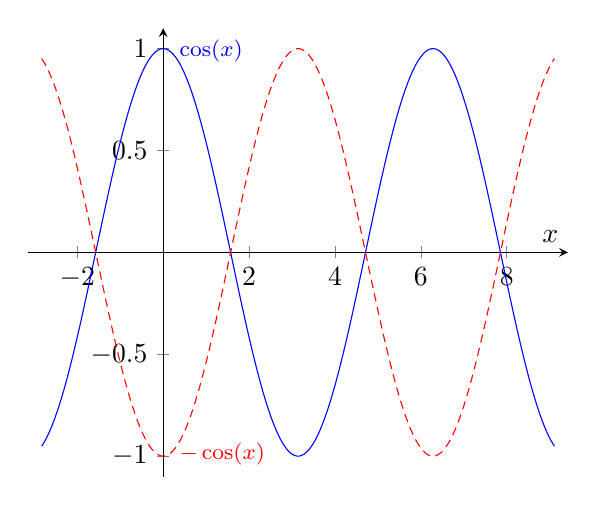
\begin{tikzpicture}
\begin{axis}[
axis lines=middle,
clip=false,
xmin=-pi,
xmax=3*pi,
ymin=-1.1,
ymax=1.1,
xlabel=$x$,
%ylabel=$y$,
xticklabel style={black}
]

\addplot[domain=-.9*pi:2.9*pi,samples=200,blue]{cos(deg(x))}
node[right,pos=.25,font=\footnotesize]{$\cos(x)$};

\addplot[domain=-.9*pi:2.9*pi,samples=200,red,densely dashed]{-cos(deg(x))}
node[right,pos=.25,font=\footnotesize]{$-\cos(x)$};

\end{axis}
\end{tikzpicture}

\end{minipage}

\bigskip
\textbf{f)} $f_3(x)= \tan x$

\begin{minipage}{\linewidth}
\centering

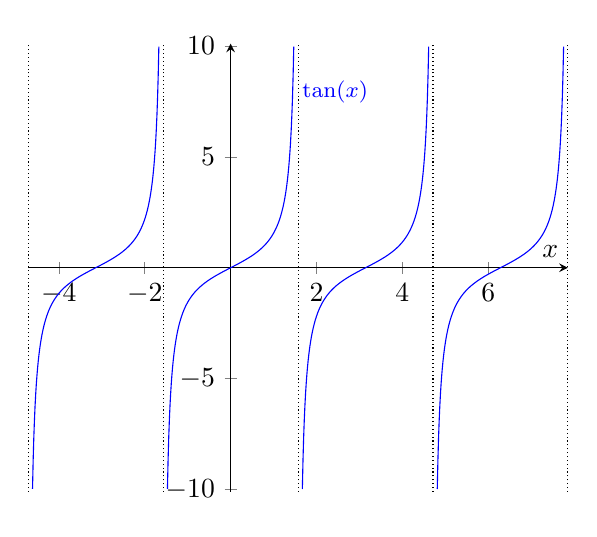
\begin{tikzpicture}
\begin{axis}[
axis lines=middle,
clip=false,
xmin=-1.5*pi,
xmax=2.5*pi,
ymin=-10.1,
ymax=10.1,
xlabel=$x$,
%ylabel=$y$,
xticklabel style={black}
]

\addplot[mark=none,black,densely dotted] coordinates {(-pi/2-pi, -10.1) (-pi/2-pi, 10.1)};

\addplot[domain=-pi/2+.1-pi:pi/2-.1-pi,samples=200,blue]{tan( deg(x) )};

\addplot[mark=none,black,densely dotted] coordinates {(-pi/2, -10.1) (-pi/2, 10.1)};

\addplot[domain=-pi/2+.1:pi/2-.1,samples=200,blue]{tan( deg(x) )}
node[right,pos=0.9,font=\footnotesize]{$\tan(x)$};

\addplot[mark=none,black,densely dotted] coordinates {(-pi/2+pi, -10.1) (-pi/2+pi, 10.1)};

\addplot[domain=-pi/2+.1+pi:pi/2-.1+pi,samples=200,blue]{tan( deg(x) )};

\addplot[mark=none,black,densely dotted] coordinates {(-pi/2+2*pi, -10.1) (-pi/2+2*pi, 10.1)};

\addplot[domain=-pi/2+.1+2*pi:pi/2-.1+2*pi,samples=200,blue]{tan( deg(x) )};

\addplot[mark=none,black,densely dotted] coordinates {(-pi/2+3*pi, -10.1) (-pi/2+3*pi, 10.1)};

\end{axis}
\end{tikzpicture}

\end{minipage}


\newpage
\bigskip
\textbf{g)} $g_1(x)=\sqrt{x}$

\begin{minipage}{\linewidth}
\centering

\begin{tikzpicture}
\begin{axis}[
axis lines=middle,
clip=false,
xmin=-1.1,
xmax=3.9,
ymin=-1.1,
ymax=3.9,
xlabel=$x$,
ylabel=$f(x)$,
xticklabel style={black}
]

\addplot[domain=0:3.7,samples=200,blue]{sqrt(x)}
node[right,pos=.1,font=\footnotesize]{$\sqrt{x}$};

\end{axis}
\end{tikzpicture}

\end{minipage}


\bigskip
\textbf{h)} $g_2(x)=\displaystyle \frac{1}{x}$

\bigskip
\textbf{i)} $g_3(x)=\displaystyle \frac{1}{x^2}$

\begin{minipage}{\linewidth}
\centering

\begin{tikzpicture}
\begin{axis}[
axis lines=middle,
clip=false,
xmin=-4.9,
xmax=4.9,
ymin=-3.9,
ymax=3.9,
xlabel=$x$,
%ylabel=$f(x)$,
xticklabel style={black}
]

\addplot[domain=-4.7:-0.3,samples=200,blue]{1/x}
node[left,pos=.7,font=\footnotesize]{$\displaystyle \frac{1}{x}$};

\addplot[domain=0.3:4.7,samples=200,blue]{1/x}
node[left,pos=.3,font=\footnotesize]{$\displaystyle \frac{1}{x}$};


\addplot[domain=-4.7:-0.54,samples=200,red,densely dashed]{1/x^2}
node[left,pos=.7,font=\footnotesize]{$\displaystyle \frac{1}{x^2}$};

\addplot[domain=0.54:4.7,samples=200,red,densely dashed]{1/x^2};

\end{axis}
\end{tikzpicture}

\end{minipage}


\newpage
\bigskip
\textbf{j)} $h_1(x)=\ln x$

\begin{minipage}{\linewidth}
\centering

\begin{tikzpicture}
\begin{axis}[
axis lines=middle,
clip=false,
xmin=-1.1,
xmax=3.9,
ymin=-3.9,
ymax=3.9,
xlabel=$x$,
ylabel=$f(x)$,
xticklabel style={black}
]

\addplot[domain=0.025:3.7,samples=200,blue]{ln(x)}
node[right,pos=.1,font=\footnotesize]{$\ln(x)$};

\end{axis}
\end{tikzpicture}

\end{minipage}


\bigskip
\textbf{k)} $h_2(x)=\ln x +1$

\begin{minipage}{\linewidth}
\centering

\begin{tikzpicture}
\begin{axis}[
axis lines=middle,
clip=false,
xmin=-1.1,
xmax=3.9,
ymin=-3.9,
ymax=3.9,
xlabel=$x$,
ylabel=$f(x)$,
xticklabel style={black}
]

\addplot[domain=0.025:3.7,samples=200,blue]{ln(x)+1}
node[right,pos=.1,font=\footnotesize]{$\ln(x)+1$};

\addplot[domain=0:3.7,black,densely dotted]{1.0};

\end{axis}
\end{tikzpicture}

\end{minipage}


\newpage
\bigskip
\textbf{l)} $h_3(x)=\ln(x+1)$


\begin{minipage}{\linewidth}
\centering

\begin{tikzpicture}
\begin{axis}[
axis lines=middle,
clip=false,
xmin=-1.1,
xmax=3.9,
ymin=-3.9,
ymax=3.9,
xlabel=$x$,
ylabel=$f(x)$,
xticklabel style={black}
]

\addplot[domain=0.025-1:3.7,samples=200,blue]{ln(x+1)}
node[right,pos=.1,font=\footnotesize]{$\ln(x+1)$};

\addplot[mark=none,black,densely dotted] coordinates {(-1, -3.9) (-1, 0)};

\end{axis}
\end{tikzpicture}

\end{minipage}
}
\ifthenelse{\boolean{mitLoes}}{\cleardoublepage}{}
\Aufgabe[f]{Vektorwertige Funktionen}{
Gegeben sei die vektorwertige Funktion $\vec f : \mathbb{R}^2 \to \mathbb{R}^2$ durch

\begin{align*}
\vec f(x_1 , x_2) = \begin{bmatrix} x_1 + 2x_2 \\ -x_1 + x_2\end{bmatrix}
\end{align*}

Zeigen Sie, dass die Funktion $\vec f$ bijektiv ist und bestimmen Sie die Inverse.
}

\Loesung{
Die Abbildung $\vec f : \mathbb{R}^2 \to \mathbb{R}^2$ kann äquivalent über die Matrix-Vektor Multiplikation $\vec A \vec x$ der Form

$$
\vec A \vec x = \begin{bmatrix}
1 & 2 \\ -1 & 1
\end{bmatrix} \begin{pmatrix}
x_1 \\ x_2
\end{pmatrix}
$$

dargestellt werden. \\ \\
%
%
%
Die inverse Abbildung ist entsprechend über die zu der Matrix $\vec A$ inverse Matrix $\vec A^{-1}$ gegeben, die sich für eine $2\times 2$-Matrix mittels

\begin{align}
\label{eq_inv}
\vec A^{-1} = \frac{1}{\text{det}(\vec A)} \begin{bmatrix}
a_{22} & -a_{21} \\ -a_{12} & a_{11}
\end{bmatrix}
\end{align}
%
%
%
berechnen lässt. \\ \\
%
%
Bevor die Inverse bestimmt wird, sollte erst geprüft werden, wann und unter welchen Umständen die Inverse existiert. Dazu gibt es die folgenden Interpretationen,
deren Bedeutungen zueinander jedoch äquivalent sind:

\begin{iii}
\item $\vec f(\vec x)$ ist bijektiv
\item $\vec A$ hat vollen Rang
\item $\vec A$ ist regulär
\item $\text{det}(\vec A) \neq 0$
\item In Gl. (\ref{eq_inv}) wird nicht durch 0 geteilt
\end{iii}

Da die Determinante ohnehin benötigt wird, berechnen wir diese zuerst mit

$$
\text{det}(\vec A) = a_{11} \cdot a_{22} - a_{21} \cdot a_{12} = 1 \cdot 1 - (-1) \cdot 2 = 3 \neq 0 \qquad \forall \vec x \in \mathbb{R} 
$$

Dementsprechend wurde gezeigt, dass die Inverse $\vec A^{-1}$ existiert und somit $\vec f(x)$ bijektiv ist. Die Inverse $\vec A^{-1}$ ergibt sich nach Gl. (\ref{eq_inv}) 
zu

$$
\vec A^{-1} =  \frac{1}{\text{det}(\vec A)} \begin{bmatrix}
a_{22} & -a_{21} \\ -a_{12} & a_{11}
\end{bmatrix} 
= \frac{1}{3} \begin{bmatrix}
1 & -2 \\ 1 & 1
\end{bmatrix}
$$

Wir prüfen dies, indem wir Inverse mit der ursprünglichen Abbildung multiplizieren.

$$
\vec A^{-1} \vec A = \frac{1}{3} \begin{bmatrix}
1 & -2 \\ 1 & 1
\end{bmatrix} 
\begin{bmatrix}
1 & 2 \\ -1 & 1
\end{bmatrix} =
\frac{1}{3} \begin{bmatrix}
3 & 0 \\ 0 & 3
\end{bmatrix} = \begin{bmatrix}
1 & 0 \\ 0 & 1
\end{bmatrix} = \vec I
$$

Dies bestätigt das berechnete Ergebnis.

Alternativ kann die Inverse mit dem Gauß-Algorithmus berechnet werden.
}


\ifthenelse{\boolean{mitLoes}}{\cleardoublepage}{}
\ifthenelse{\boolean{mitErg}}{
\ruleBig
\Ergebnisse}{}


\end{twocolumn}
\end{document}
